\documentclass[10pt,a4paper]{article}
\usepackage[margin=1.6cm]{geometry}
\usepackage{booktabs}
\usepackage{array}
\usepackage{tikz}
\usetikzlibrary{arrows.meta,positioning,shapes.geometric}
\usepackage{enumitem}
\usepackage{xcolor}
\usepackage{tcolorbox}
\usepackage{hyperref}
\usepackage{amsmath}
\usepackage{parskip}

\hypersetup{colorlinks=true,linkcolor=blue!60!black,urlcolor=blue!60!black}

\title{\vspace{-2em}License Plate Deblurring --- Presentation Cheat Sheet}
\author{Group ``Opus'': Hamza Ziouine \& Leonce Theureau \\ S8 Introduction to Computer Vision --- UIR}
\date{}

\setlist[itemize]{leftmargin=*,itemsep=1pt,topsep=2pt}
\setlist[enumerate]{leftmargin=*,itemsep=1pt,topsep=2pt}

\newtcolorbox{qabox}[1]{colback=blue!3,colframe=blue!40!black,boxrule=0.4pt,left=4pt,right=4pt,top=2pt,bottom=2pt,fonttitle=\bfseries\small,title={#1}}

\begin{document}
\maketitle
\vspace{-2.2em}

% =========================================================================
\section*{1. Project in One Paragraph}
A \textbf{classical, learning-free} pipeline for restoring blurred license
plate images: blind PSF estimation from the log-magnitude FFT, five
deconvolution methods, and PSNR/SSIM evaluation on a synthetic 3\,003-pair
dataset. Total Variation denoising is an \emph{optional post-process}
(not in headline metrics); OCR is \emph{future work}.

% =========================================================================
\section*{2. Pipeline (headline path)}
\begin{center}
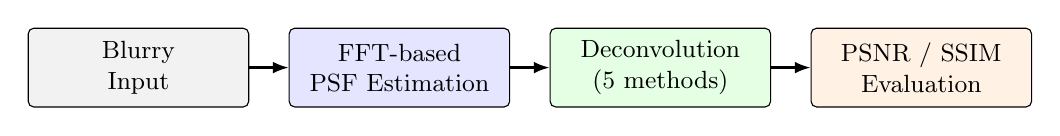
\begin{tikzpicture}[
  node distance=6mm and 5mm,
  box/.style={draw,rounded corners=2pt,minimum height=10mm,minimum width=28mm,align=center,font=\small},
  arr/.style={-{Latex[length=2mm]},thick}
]
\node[box,fill=gray!10] (in) {Blurry\\Input};
\node[box,fill=blue!10,right=of in] (psf) {FFT-based\\PSF Estimation};
\node[box,fill=green!10,right=of psf] (dec) {Deconvolution\\(5 methods)};
\node[box,fill=orange!10,right=of dec] (ev) {PSNR / SSIM\\Evaluation};
\draw[arr] (in) -- (psf);
\draw[arr] (psf) -- (dec);
\draw[arr] (dec) -- (ev);
\end{tikzpicture}
\end{center}
\textbf{Not in headline:} TV denoising (optional post), OCR (future work).

% =========================================================================
\section*{3. Glossary (memorize)}
\begin{itemize}
  \item \textbf{PSF} --- Point Spread Function: the blur kernel $h$ such that $b = h \ast x + n$.
  \item \textbf{FFT} --- Fast Fourier Transform: frequency-domain representation; convolution becomes multiplication.
  \item \textbf{PSNR} --- Peak Signal-to-Noise Ratio, in dB; higher is better.
  \item \textbf{SSIM} --- Structural Similarity index, in $[0,1]$; higher is better.
  \item \textbf{SNR} --- Signal-to-Noise Ratio.
  \item \textbf{CLS} --- Constrained Least Squares: Tikhonov with Laplacian regularizer (pedagogical baseline).
  \item \textbf{RL} --- Richardson--Lucy: iterative Bayesian deconvolution under Poisson noise.
  \item \textbf{TV} --- Total Variation regularization (optional post-processing denoiser).
  \item \textbf{OCR} --- Optical Character Recognition (future work, \emph{not} evaluated here).
\end{itemize}

% =========================================================================
\section*{4. Five Deconvolution Methods}
\begin{enumerate}
  \item \textbf{Inverse} --- $\hat X = B / H$. Pedagogical baseline; explodes on noise \& zeros of $H$.
  \item \textbf{Wiener} --- MMSE filter $\hat X = \overline{H} B / (|H|^2 + K)$. \textbf{Best performer} here.
  \item \textbf{Unsupervised Wiener} --- Wiener with Gibbs-sampled noise/signal variance estimation (no manual $K$).
  \item \textbf{Richardson--Lucy} (30 iters) --- iterative Bayesian under Poisson noise; non-negative.
  \item \textbf{CLS} ($\gamma{=}0.01$) --- Tikhonov with Laplacian regularizer; pedagogical.
\end{enumerate}

% =========================================================================
\section*{5. Dataset}
\begin{itemize}
  \item \textbf{3\,003 pairs} generated from \textbf{1\,001 clean plates}.
  \item Splits \textbf{2100 / 450 / 453} (train / val / test). \textbf{No leakage by source image.}
  \item \textbf{Blur}: Gaussian $\sigma \in [1,5]$; motion length $\in [5,25]\,\text{px}$; defocus radius $\in [3,10]\,\text{px}$.
  \item \textbf{Degradation}: additive noise $\sigma \in [5,15]$, JPEG quality $\in [50,85]$.
\end{itemize}

\newpage
% =========================================================================
\section*{6. Results --- Motion Subset (151 images, blind PSF)}
\begin{center}
\begin{tabular}{lrr}
\toprule
\textbf{Method} & \textbf{PSNR (dB)} & \textbf{SSIM} \\
\midrule
Blurry (input baseline)        & 23.03 & 0.577 \\
Wiener                         & 14.64 & 0.189 \\
Richardson--Lucy ($n{=}30$)    & 12.67 & 0.163 \\
Unsupervised Wiener            & 10.88 & 0.082 \\
CLS ($\gamma{=}0.01$)          & 10.26 & 0.033 \\
Inverse                        &  9.61 & 0.009 \\
\bottomrule
\end{tabular}
\end{center}

\begin{tcolorbox}[colback=red!5,colframe=red!60!black,boxrule=0.4pt,title=\textbf{Headline (say this first)}]
\textbf{All blind classical methods fall \emph{below} the blurry baseline on motion blur.}
Best (Wiener) is $\mathbf{-8.4\,\text{dB}}$ PSNR vs input. The \textbf{oracle-PSF}
sanity check (known kernel, $n{=}1$ example) gives $\mathbf{+2.2\,\text{dB}}$ ---
the deconvolution code is correct; the \textbf{bottleneck is blind PSF estimation}.
Oracle-vs-blind gap on motion: $\sim \mathbf{10.6\,\text{dB}}$.
\end{tcolorbox}

\begin{tcolorbox}[colback=yellow!8,colframe=orange!70!black,boxrule=0.4pt,title=\textbf{Surprise finding}]
\textbf{Wiener performs better on defocus (16.72 dB) than on motion (14.64 dB),}
even though motion was our target regime. \textbf{Why:} motion-blur PSFs have
directional \emph{nulls} in frequency; a small error in estimated angle puts
those nulls in the wrong place, catastrophically amplifying the wrong frequencies.
Defocus PSFs are isotropic (no preferred direction), so angle error is irrelevant
and the spectrum is more forgiving.
\end{tcolorbox}

% =========================================================================
\section*{7. Likely Q\&A (prepare answers)}

\begin{qabox}{Q1. Why are your restored images \emph{worse} than the blurry input?}
The blurry input is smooth; classical deconvolution amplifies high frequencies.
Under additive noise and JPEG quantization, the amplification multiplies the
\emph{noise}, not the signal. PSNR punishes noise amplification more than blur.
\end{qabox}

\begin{qabox}{Q2. Then how do you know your code is correct?}
Oracle experiment: with the \emph{true} PSF, Wiener gives $+2.2\,\text{dB}$ over
the blurry input. That isolates the algorithm from the PSF-estimation stage and
proves the math and implementation are correct.
\end{qabox}

\begin{qabox}{Q3. Why is CLS the worst?}
CLS uses a Laplacian (high-pass) regularizer, which assumes the solution is
smooth. This conflicts with the structure-rich plate text we want to recover,
and its fixed $\gamma$ has no mechanism to estimate noise --- so it over-sharpens
artifacts.
\end{qabox}

\begin{qabox}{Q4. Wiener vs.\ Richardson--Lucy --- why does Wiener win?}
Wiener is a closed-form MMSE filter tuned for \emph{Gaussian} noise, which matches
our degradation. RL assumes \emph{Poisson} noise (photon-counting model); it is
mismatched here, and its iterative amplification diverges earlier under PSF error.
\end{qabox}

\begin{qabox}{Q5. What does the oracle result actually mean?}
It is an upper bound on what our deconvolution back-end can deliver \emph{given
a perfect kernel}. The $\sim 10.6\,\text{dB}$ gap between oracle and blind on
motion is the cost of PSF-estimation error --- the real research problem.
\end{qabox}

\begin{qabox}{Q6. Why did noise and JPEG hurt so much?}
JPEG quantization destroys high-frequency content in $8{\times}8$ blocks --- the
exact band that carries thin character strokes. Deconvolution then amplifies
quantization artifacts rather than plate detail. Noise compounds this linearly
in the frequency domain.
\end{qabox}

\begin{qabox}{Q7. Why are motion-blur PSFs especially hard?}
A motion-blur PSF in frequency has \emph{zeros along a line perpendicular to
motion direction}. Any error in the estimated angle places those zeros in the
wrong direction, and dividing by near-zero frequencies in the wrong places
creates the worst possible artifacts.
\end{qabox}

\begin{qabox}{Q8. Why no TV ablation, no OCR?}
TV denoising is scoped as an \emph{optional post-process} and is not in the
headline numbers. OCR / CER evaluation is future work: blind restorations are
below baseline, so OCR would not add information for the core claim.
\end{qabox}

\begin{qabox}{Q9. Known limitations}
Blind methods below baseline under noise + JPEG; oracle is a single example
($n{=}1$); no OCR / CER evaluation; no TV on/off ablation; means-only reporting
(no per-image variance); PSF estimation from log-magnitude FFT is sensitive to noise.
\end{qabox}

% =========================================================================
\section*{8. Code Structure (do not swap!)}
\begin{itemize}
  \item \texttt{src/blur\_generator.py} --- \textbf{blur synthesis + degradation} (Gaussian / motion / defocus PSFs; additive noise; JPEG compression).
  \item \texttt{src/classical\_deblur.py} --- \textbf{five deconvolution methods} + TV post + PSF builder utilities.
  \item \texttt{code/pipeline.ipynb} --- end-to-end \textbf{demo + evaluation} notebook (metrics, figures).
\end{itemize}

% =========================================================================
\section*{9. One-Sentence Summary}
\emph{``Our blind classical pipeline implements five deconvolution methods
correctly --- the oracle sanity check proves it --- but under realistic noise
and JPEG, blind PSF estimation error dominates, and all methods fall below the
blurry baseline; the $\sim 10.6\,\text{dB}$ oracle gap on motion blur is the
honest measurement of the classical approach's limit.''}

\end{document}
